\chapter{Magic methods}
\subsection{Introduction}
Now that we have discussed both functions and classes, we can proceed to one of the features where Python really differs from e.g. JavaScript, namely the so called magic methods. These magic methods can be thought of as hooks, that allows the programmer to get to execute code at e.g. attribute access. We already showed in the section about classes how to handle the magic method \inlinecode{\_\_init\_\_}. This particular magic method is less interesting from many other magic methods, as it just corresponds to a constructor.

Two very important magic methods, however, are \inlinecode{\_\_getattribute\_\_} and \inlinecode{\_\_getattr\_\_}. Each time a attribute \inlinecode{a} is read from a class object \inlinecode{x}, the following happens:

The magic method \inlinecode{\_\_getattribute\_\_} is looked up on \inlinecode{x}. If it is defined, the method is called with the instance, \inlinecode{x}, and the attribute name \inlinecode{a}. It is now up to the supplied method to return the correct value. If the implementation of \inlinecode{\_\_getattribute\_\_} happens to raise an \inlinecode{AttributeError}, \inlinecode{\_\_getattr\_\_} is called. Otherwise if \inlinecode{\_\_getattribute\_\_} is not defined, the attribute is looked up on the instance. If the attribute is present on the instance it is returned, otherwise an \inlinecode{AttributeError} is raised and the magic method \inlinecode{\_\_getattr\_\_} is called (at least if it is defined).

Thus, the magic method \inlinecode{\_\_getattribute\_\_} can be used to supply a custom attribute lookup function, and \inlinecode{\_\_getattr\_\_} can be used to supply a fallback function in case of a bad attribute access. Note also that the \inlinecode{\_\_getattribute\_\_} can not be thought of as being equivalent (or nearly equivalent) to getters in e.g. ECMAScript 5 and C\#: In Python one single method is supplied, not one for each attribute (or property and field for ECMAScript 5, respectively C\#).

Because of the limited time of our project we have not been able to support both \inlinecode{\_\_getattribute\_\_} and \inlinecode{\_\_getattr\_\_} in our implementation. Instead, we looked at the use of these magic methods in some larger Python projects, in order to determine which seemed most useful and important to support. In Django 1.5.1\footnote{See \url{http://www.djangoproject.com/}.}, a high-level web framework, we found that \inlinecode{\_\_getattribute\_\_} was not used at all. However, \inlinecode{\_\_getattr\_\_} is used 14 times. Of course this is not much for a web framework on approximately 200.000 lines of code, but it is still essential to handle in order to be able to statically analyze Python programs.

\subsection{Transforming the CFG}
Since each single attribute access possibly involves method calls, we normalize the CFG in order to reflect this. More concretely, we normalize each node in the CFG of the following form: \inlinecode{<res>=ReadProperty(<base>,prop)}, into the following CFG piece:

%\begin{listing}[H]
%	\begin{center}
%		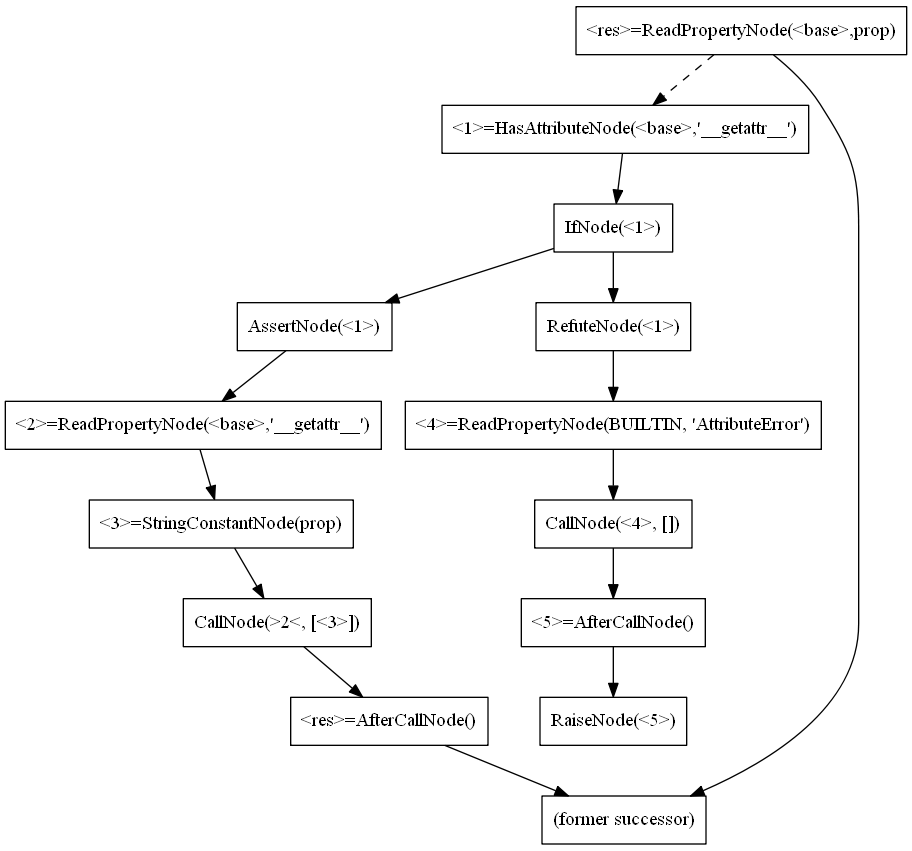
\includegraphics[width=0.75\textwidth]{images/readproperty.png}
%	\end{center}
%	\vspace{-10pt}
%	\caption{The normalization of a read property node.}
%	\label{fig:ReadPropertyCFG}
%\end{listing}

As can be seen from the normalized CFG of read property nodes the only challenge there is in order for our analysis to handle the magic method \inlinecode{\_\_getattr\_\_}, is that we need to handle exceptions in our analysis. We return to this in the following section. First, we want to note the following thing about our normalization: If an attribute is definately set on an instance object, \inlinecode{\_\_getattr\_\_} is never called when reading that particular property. This is the case as there won't be any flow across the exception edge in the figure above, because the \inlinecode{ReadPropertyNode} will always succeed in reading the attribute and therefore not raise any \inlinecode{AttributeError}.

Thus the analysis can be improved such that it only normalizes read property nodes if the read property may not be defined (resulting in possibly $12 * \#\texttt{read property nodes}$ nodes less in the CFG). This is exactly what our implementation does. In order to obtain this we have provided the analysis with an interface to the worklist algorithm, such that our type analysis tool can modify the control flow graph. When doing this, each newly added node to the CFG must of course be added to the worklist.
